\section{Shap}

\begin{frame}
	\begin{block}{Artigo 03}
	\begin{enumerate}
		\item Consistent Individualized Feature Attribution for Tree Ensembles \cite{SHAP}
	\end{enumerate}
	\end{block}
\end{frame}


\begin{frame}
	\begin{block}{Shap - overview}
		\begin{enumerate}
			\item Não é agnóstico (funciona apenas para ensemble de árvore de decisão)
			\item Realiza uma interpretação Local do score gerado pelo modelo.
			\item Citam o problema de incosistência (score alto para variáveis que não são importantes e o caso contrário) 
			\item Um ponto falho é que o SHAP foi avaliado perguntando para algumas pessoas (os autores não citam esse número ) quais features eram mais relevantes.
		\end{enumerate}
	\end{block}
\end{frame}

\begin{frame}
	\begin{block}{Shap - funcionamento}
			\begin{enumerate}
				\item Realiza uma perturbação do dado de entrada, roda um modelo aditivo sobre o dado orignal e sobre o perturbado.
				\item Interpreta o modelo aditivo para dizer o quanto a variável foi explicativa para aquela decisão
				\item A diferença em relação ao LIME é que no modelo aditivo encontro o phi (equivalente ao beta da regressão) com probabilidade condicional, a logística usa uma técnica de otimização  (e.g. Least square)
			\end{enumerate}
	\end{block}
\end{frame}

\begin{frame}
	\begin{block}{SHAP - output}
		\begin{figure}[!htb]
			\centering	  				
			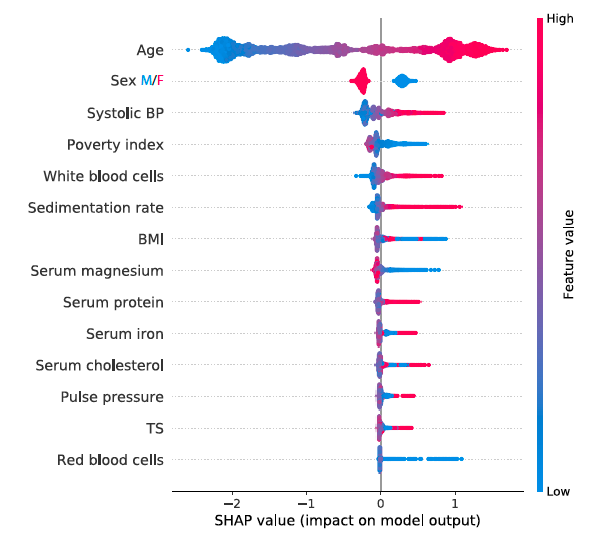
\includegraphics[height=4cm, width = 7cm]{./pic/shapModel.png}
			\caption{SHAP - output \cite{SHAP}}
			\label{fig_ds_process}
		\end{figure}	
	\end{block}
\end{frame}

